%%
%% Automatically generated file from DocOnce source
%% (https://github.com/hplgit/doconce/)
%%

% #define PREAMBLE

% #ifdef PREAMBLE
%-------------------- begin preamble ----------------------

\documentclass[%
oneside,                 % oneside: electronic viewing, twoside: printing
final,                   % draft: marks overfull hboxes, figures with paths
10pt]{article}

\listfiles               %  print all files needed to compile this document

\usepackage{relsize,makeidx,color,setspace,amsmath,amsfonts,amssymb}
\usepackage[table]{xcolor}
\usepackage{bm,ltablex,microtype}

\usepackage[pdftex]{graphicx}

% Packages for typesetting blocks of computer code
\usepackage{fancyvrb,framed,moreverb}

% Define colors
\definecolor{orange}{cmyk}{0,0.4,0.8,0.2}
\definecolor{tucorange}{rgb}{1.0,0.64,0}
\definecolor{darkorange}{rgb}{.71,0.21,0.01}
\definecolor{darkgreen}{rgb}{.12,.54,.11}
\definecolor{myteal}{rgb}{.26, .44, .56}
\definecolor{gray}{gray}{0.45}
\definecolor{mediumgray}{gray}{.8}
\definecolor{lightgray}{gray}{.95}
\definecolor{brown}{rgb}{0.54,0.27,0.07}
\definecolor{purple}{rgb}{0.5,0.0,0.5}
\definecolor{darkgray}{gray}{0.25}
\definecolor{darkblue}{rgb}{0,0.08,0.45}
\definecolor{darkblue2}{rgb}{0,0,0.8}
\definecolor{lightred}{rgb}{1.0,0.39,0.28}
\definecolor{lightgreen}{rgb}{0.48,0.99,0.0}
\definecolor{lightblue}{rgb}{0.53,0.81,0.92}
\definecolor{lightblue2}{rgb}{0.3,0.3,1.0}
\definecolor{lightpurple}{rgb}{0.87,0.63,0.87}
\definecolor{lightcyan}{rgb}{0.5,1.0,0.83}

\colorlet{comment_green}{green!50!black}
\colorlet{string_red}{red!60!black}
\colorlet{keyword_pink}{magenta!70!black}
\colorlet{indendifier_green}{green!70!white}

% Backgrounds for code
\definecolor{cbg_gray}{rgb}{.95, .95, .95}
\definecolor{bar_gray}{rgb}{.92, .92, .92}

\definecolor{cbg_yellowgray}{rgb}{.95, .95, .85}
\definecolor{bar_yellowgray}{rgb}{.95, .95, .65}

\colorlet{cbg_yellow2}{yellow!10}
\colorlet{bar_yellow2}{yellow!20}

\definecolor{cbg_yellow1}{rgb}{.98, .98, 0.8}
\definecolor{bar_yellow1}{rgb}{.98, .98, 0.4}

\definecolor{cbg_red1}{rgb}{1, 0.85, 0.85}
\definecolor{bar_red1}{rgb}{1, 0.75, 0.85}

\definecolor{cbg_blue1}{rgb}{0.87843, 0.95686, 1.0}
\definecolor{bar_blue1}{rgb}{0.7,     0.95686, 1}

\usepackage{listingsutf8}

% Common lstlisting parameters

\usepackage{calc}
\newlength{\lstboxwidth}  % width of lst box
\newlength{\framethickness}
\setlength{\framethickness}{0.5mm}
% for frame=trbl and a framerule that has significant size, set
% xleftmargin=5mm and xrightmargin=5mm.

\lstset{
  basicstyle=\small \ttfamily,
  breaklines=false,          % break/wrap lines
  breakatwhitespace=true,    % let linebreaks happen at whitespace
  breakindent=40pt,
  tab=,
  tabsize=4,                 % tab means 4 spaces
  %belowskip=\smallskipamount,  % space between code and text below
  xleftmargin=2mm,           % indentation of code frame
  xrightmargin=0mm,
  framexleftmargin=2mm,      % add frame space to the left of the code box
  %numbers=left,             % put line numbers on the left
  %stepnumber=2,             % stepnumber=1 numbers each line, =n every n lines
  framerule=\framethickness, % thickness of frame
  aboveskip=2ex,             % vertical space above code frame
  showstringspaces=false,    % show spaces in strings with an underscore
  showspaces=false,          % show spaces with an underscore
  showtabs=false,
  keepspaces=true,
  columns=fullflexible,      % tighter character kerning, like verb
  escapeinside={(*@}{@*)},   % (*@ \pause @*) in slides and math in code blocks
  extendedchars=\true,       % allows non-ascii chars, does not work with utf-8
}

% Internally defined styles for lstlisting

% Use this one without additional background color
\lstdefinestyle{blue1}{              % blue1 background for code snippets
backgroundcolor=\color{cbg_blue1},
}

% Use this one without additional background color
% (same as blue1, but with bar_blue1 frame)
\lstdefinestyle{blue1bar}{           % blue1 background for complete programs
backgroundcolor=\color{cbg_blue1},
frame=tb,                            % include frame
rulecolor=\color{bar_blue1},         % frame color
}

% Use this one without additional background color
\lstdefinestyle{gray}{
backgroundcolor=\color{cbg_gray},
%frame=tb,                            % include frame
%framerule=0.4pt                      % thickness of frame
rulecolor=\color{black!40},           % frame color
}

\lstdefinestyle{simple}{
commentstyle={},
}

% end of custom lstdefinestyles

\usepackage[T1]{fontenc}
%\usepackage[latin1]{inputenc}
\usepackage{ucs}
\usepackage[utf8x]{inputenc}

\usepackage{lmodern}         % Latin Modern fonts derived from Computer Modern

% Hyperlinks in PDF:
\definecolor{linkcolor}{rgb}{0,0,0.4}
\usepackage{hyperref}
\hypersetup{
    breaklinks=true,
    colorlinks=true,
    linkcolor=linkcolor,
    urlcolor=linkcolor,
    citecolor=black,
    filecolor=black,
    %filecolor=blue,
    pdfmenubar=true,
    pdftoolbar=true,
    bookmarksdepth=3   % Uncomment (and tweak) for PDF bookmarks with more levels than the TOC
    }
%\hyperbaseurl{}   % hyperlinks are relative to this root

\setcounter{tocdepth}{2}  % levels in table of contents

% Tricks for having figures close to where they are defined:
% 1. define less restrictive rules for where to put figures
\setcounter{topnumber}{2}
\setcounter{bottomnumber}{2}
\setcounter{totalnumber}{4}
\renewcommand{\topfraction}{0.95}
\renewcommand{\bottomfraction}{0.95}
\renewcommand{\textfraction}{0}
\renewcommand{\floatpagefraction}{0.75}
% floatpagefraction must always be less than topfraction!
% 2. ensure all figures are flushed before next section
\usepackage[section]{placeins}
% 3. enable begin{figure}[H] (often leads to ugly pagebreaks)
%\usepackage{float}\restylefloat{figure}

% --- fancyhdr package for fancy headers ---
\usepackage{fancyhdr}
\fancyhf{} % sets both header and footer to nothing
\renewcommand{\headrulewidth}{0pt}
\fancyfoot[LE,RO]{\thepage}
% Ensure copyright on titlepage (article style) and chapter pages (book style)
\fancypagestyle{plain}{
  \fancyhf{}
  \fancyfoot[C]{{\footnotesize \copyright\ 2018-2019, Christian Forssén. Released under CC Attribution-NonCommercial 4.0 license}}
%  \renewcommand{\footrulewidth}{0mm}
  \renewcommand{\headrulewidth}{0mm}
}
% Ensure copyright on titlepages with \thispagestyle{empty}
\fancypagestyle{empty}{
  \fancyhf{}
  \fancyfoot[C]{{\footnotesize \copyright\ 2018-2019, Christian Forssén. Released under CC Attribution-NonCommercial 4.0 license}}
  \renewcommand{\footrulewidth}{0mm}
  \renewcommand{\headrulewidth}{0mm}
}

\pagestyle{fancy}


\usepackage[framemethod=TikZ]{mdframed}

% --- begin definitions of admonition environments ---

% Admonition style "mdfbox" is an oval colored box based on mdframed
% "notice" admon
\definecolor{mdfbox_notice_background}{rgb}{1,1,1}
\newmdenv[
  skipabove=15pt,
  skipbelow=15pt,
  outerlinewidth=0,
  backgroundcolor=mdfbox_notice_background,
  linecolor=black,
  linewidth=2pt,       % frame thickness
  frametitlebackgroundcolor=mdfbox_notice_background,
  frametitlerule=true,
  frametitlefont=\normalfont\bfseries,
  shadow=false,        % frame shadow?
  shadowsize=11pt,
  leftmargin=0,
  rightmargin=0,
  roundcorner=5,
  needspace=0pt,
]{notice_mdfboxmdframed}

\newenvironment{notice_mdfboxadmon}[1][]{
\begin{notice_mdfboxmdframed}[frametitle=#1]
}
{
\end{notice_mdfboxmdframed}
}

% Admonition style "mdfbox" is an oval colored box based on mdframed
% "summary" admon
\definecolor{mdfbox_summary_background}{rgb}{1,1,1}
\newmdenv[
  skipabove=15pt,
  skipbelow=15pt,
  outerlinewidth=0,
  backgroundcolor=mdfbox_summary_background,
  linecolor=black,
  linewidth=2pt,       % frame thickness
  frametitlebackgroundcolor=mdfbox_summary_background,
  frametitlerule=true,
  frametitlefont=\normalfont\bfseries,
  shadow=false,        % frame shadow?
  shadowsize=11pt,
  leftmargin=0,
  rightmargin=0,
  roundcorner=5,
  needspace=0pt,
]{summary_mdfboxmdframed}

\newenvironment{summary_mdfboxadmon}[1][]{
\begin{summary_mdfboxmdframed}[frametitle=#1]
}
{
\end{summary_mdfboxmdframed}
}

% Admonition style "mdfbox" is an oval colored box based on mdframed
% "warning" admon
\definecolor{mdfbox_warning_background}{rgb}{1,1,1}
\newmdenv[
  skipabove=15pt,
  skipbelow=15pt,
  outerlinewidth=0,
  backgroundcolor=mdfbox_warning_background,
  linecolor=black,
  linewidth=2pt,       % frame thickness
  frametitlebackgroundcolor=mdfbox_warning_background,
  frametitlerule=true,
  frametitlefont=\normalfont\bfseries,
  shadow=false,        % frame shadow?
  shadowsize=11pt,
  leftmargin=0,
  rightmargin=0,
  roundcorner=5,
  needspace=0pt,
]{warning_mdfboxmdframed}

\newenvironment{warning_mdfboxadmon}[1][]{
\begin{warning_mdfboxmdframed}[frametitle=#1]
}
{
\end{warning_mdfboxmdframed}
}

% Admonition style "mdfbox" is an oval colored box based on mdframed
% "question" admon
\definecolor{mdfbox_question_background}{rgb}{1,1,1}
\newmdenv[
  skipabove=15pt,
  skipbelow=15pt,
  outerlinewidth=0,
  backgroundcolor=mdfbox_question_background,
  linecolor=black,
  linewidth=2pt,       % frame thickness
  frametitlebackgroundcolor=mdfbox_question_background,
  frametitlerule=true,
  frametitlefont=\normalfont\bfseries,
  shadow=false,        % frame shadow?
  shadowsize=11pt,
  leftmargin=0,
  rightmargin=0,
  roundcorner=5,
  needspace=0pt,
]{question_mdfboxmdframed}

\newenvironment{question_mdfboxadmon}[1][]{
\begin{question_mdfboxmdframed}[frametitle=#1]
}
{
\end{question_mdfboxmdframed}
}

% Admonition style "mdfbox" is an oval colored box based on mdframed
% "block" admon
\definecolor{mdfbox_block_background}{rgb}{1,1,1}
\newmdenv[
  skipabove=15pt,
  skipbelow=15pt,
  outerlinewidth=0,
  backgroundcolor=mdfbox_block_background,
  linecolor=black,
  linewidth=2pt,       % frame thickness
  frametitlebackgroundcolor=mdfbox_block_background,
  frametitlerule=true,
  frametitlefont=\normalfont\bfseries,
  shadow=false,        % frame shadow?
  shadowsize=11pt,
  leftmargin=0,
  rightmargin=0,
  roundcorner=5,
  needspace=0pt,
]{block_mdfboxmdframed}

\newenvironment{block_mdfboxadmon}[1][]{
\begin{block_mdfboxmdframed}[frametitle=#1]
}
{
\end{block_mdfboxmdframed}
}

% --- end of definitions of admonition environments ---

% prevent orhpans and widows
\clubpenalty = 10000
\widowpenalty = 10000

% --- end of standard preamble for documents ---


\usepackage[swedish]{babel}

\raggedbottom
\makeindex
\usepackage[totoc]{idxlayout}   % for index in the toc
\usepackage[nottoc]{tocbibind}  % for references/bibliography in the toc

%-------------------- end preamble ----------------------

\begin{document}

% matching end for #ifdef PREAMBLE
% #endif

\newcommand{\exercisesection}[1]{\subsection*{#1}}

\input{newcommands_keep}

% ------------------- main content ----------------------



% ----------------- title -------------------------

\thispagestyle{empty}

\begin{center}
{\LARGE\bf
\begin{spacing}{1.25}
Learning from data: Error propagation and nuisance parameters
\end{spacing}
}
\end{center}

% ----------------- author(s) -------------------------

\begin{center}
{\bf Christian Forssén}
\end{center}

    \begin{center}
% List of all institutions:
\centerline{{\small Department of Physics, Chalmers University of Technology, Sweden}}
\end{center}
    
% ----------------- end author(s) -------------------------

% --- begin date ---
\begin{center}
Sep 24, 2019
\end{center}
% --- end date ---

\vspace{1cm}


% !split
\section{Why Bayes is Better}

\paragraph{Quotes from one pioneering and one renaissance Bayesian authority.}
Laplace:

\begin{quote}
\emph{"Probability theory is nothing but common sense reduced to calculation."}
\end{quote}


Sivia

\begin{quote}
\emph{"Bayesian inference probabilities are a measure of our state of knowledge about nature, not a measure of nature itself."}
\end{quote}


% !split
\subsection{Advantages of the Bayesian approach}
% !bpop
\begin{enumerate}
\item Provides an elegantly simple and rational approach for answering, in an optimal way, any scientific question for a given state of information. This contrasts to the recipe or cookbook approach of conventional statistical analysis. The procedure is well-defined:
\begin{itemize}

  \item Clearly state your question and prior information.

  \item Apply the sum and product rules. The starting point is always Bayes’ theorem.

\end{itemize}

\noindent
\item For some problems, a Bayesian analysis may simply lead to a familiar statistic. Even in this situation it often provides a powerful new insight concerning the interpretation of the statistic.

\item Incorporates relevant prior (e.g., known signal model or known theory model expansion) information through Bayes’ theorem. This is one of the great strengths of Bayesian analysis.
\begin{itemize}

  \item For data with a small signal-to-noise ratio, a Bayesian analysis can frequently yield many orders of magnitude improvement in model parameter estimation, through the incorporation of relevant prior information about the signal model.

\end{itemize}

\noindent
\item Provides a way of eliminating nuisance parameters through marginalization. For some problems, the marginalization can be performed analytically, permitting certain calculations to become computationally tractable.

\item Provides a way for incorporating the effects of systematic errors arising from both the measurement operation and theoretical model predictions.

\item Calculates probability of hypothesis directly: $p(H_i|D, I)$.

\item Provides a more powerful way of assessing competing theories at the forefront of science by automatically quantifying Occam’s razor.
\end{enumerate}

\noindent
% !epop

% !split
The Bayesian quantitative Occam’s razor can also save a lot of time that might otherwise be spent chasing noise artifacts that masquerade as possible detections of real phenomena.

% !split
\paragraph{Occam's razor.}
Occam’s razor is a principle attributed to the medieval philosopher William of Occam (or Ockham). The principle states that one should not make more assumptions than the minimum needed. It underlies all scientific modeling and theory building. It cautions us to choose from a set of otherwise equivalent models of a given phenomenon the simplest one. In any given model, Occam’s razor helps us to "shave off" those variables that are not really needed to explain the phenomenon. It was previously thought to be only a qualitative principle.

% !split

\begin{figure}[!ht]  % 
  \centerline{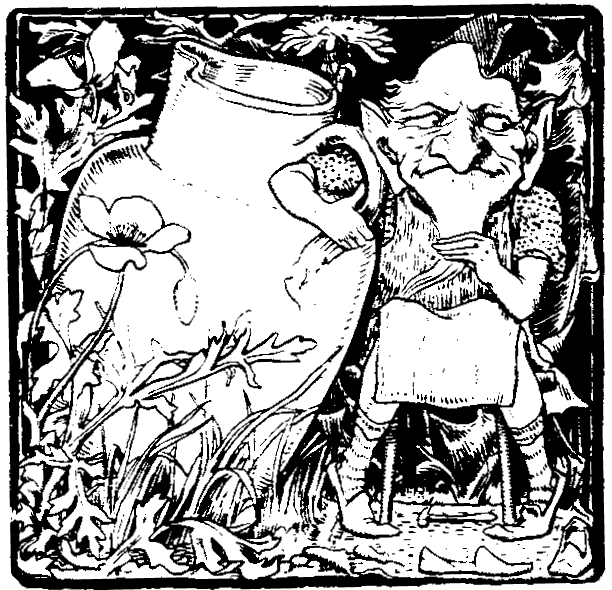
\includegraphics[width=0.7\linewidth]{fig/Leprechaun_or_Clurichaun.png}}
  \caption{
  Did the Leprechaun drink your wine, or is there a simpler explanation?
  }
\end{figure}
%\clearpage % flush figures 


% !split
\subsection{Nuisance parameters (I)}
See demonstration notebook: A Bayesian Billiard game

% !split
\subsection{Nuisance parameters (II): marginal distributions}
Assume that we have a model with two parameters, $\theta0,\theta_1$, although only one of them (say $\theta_1$) is of physical relevance (the other one is a nuisance parameter). Through a Bayesian data analysis we have the joint, posterior pdf
\[
p(\theta_0, \theta_1 | D, I).
\]
The marginal posterior pdf $p(\theta_1 | D, I)$ is obtained via marginalization
\[
p(\theta_1 | D, I) = \int p(\theta_0, \theta_1 | D, I) d\theta_0.
\]
Assume that we have $N$ samples from the joint pdf. This might be the Markov Chain from an MCMC sampler: $\left\{ (\theta_0, \theta_1)_i \right\}_{i=0}^{N-1}$. Then the marginal distribution of $\theta_1$ will be given by the same chain by simply ignoring the $\theta_0$ column, i.e., $\left\{ \theta_{1,i} \right\}_{i=0}^{N-1}$. 

See the interactive demos created by Chi Feng for an illustration of this: \href{{https://chi-feng.github.io/mcmc-demo/}}{The Markov-chain Monte Carlo Interactive Gallery}.

% !split
\subsection{Error propagation (I): marginalization}
The Bayesian approach offers a straight-forward approach for dealing with (known) systematic uncertainties; namely by marginalization. Let us demonstrate this with an example \\

% !split
\textbf{Inferring galactic distances with an imprecise knowledge of the Hubble constant}
The Hubble constant acts as a galactic ruler as it is used to measure astronomical distances according to $v = H_0 x$. An error in this ruler will therefore correspond to a systematic uncertainty in such measurements.

Here we use marginalization to obtain the desired posterior pdf $p(x|D,I)$ from the joint distribution of $p(x,H_0|D,I)$
\begin{equation}
p(x|D,I) = \int_{-\infty}^\infty dH_0 p(x,H_0|D,I).
\label{eq:marginalization}
\end{equation}

Using Bayes' rule: $p(x,H_0|D,I) \propto p(D|x,H_0,I) p(x,H_0|I)$, the product rule: $p(x,H_0|I) = p(H_0|x,I)p(x|I)$, and the fact that $H_0$ is independent of $x$: $p(H_0|x,I) = p(H_0|I)$, we find that
\[
p(x|D,I) \propto p(x|I) \int dH_0 p(H_0|I) p(D|x,H_0,I),
\]
which means that we have expressed the quantity that we want (the posterior of $x$) in terms of quantities that we know.

Assume that the pdf $p(H_0 | I)$ is known via its $N$ samples $\{H_{i}\}_{i=0}^{N-1}$ generated by the MCMC sampler.

This means that we can approximate 
\[
p(x |D,I) \propto \int dH_0 p(H_0|I) p(D|x,H_0,I) \approx \frac{1}{N} \sum_{i=1}^N p(D | x, H_i, I)
\]
where we have used a uniform prior for the distance $p(x|I) \propto 1$.


% !split
\subsection{Error propagation (II): changing variables and prior information}
(Based on Sivia, ch 3.6.)

Assume that we have measured parameter $X = 10 \pm 3$ and $Y=7 \pm 2$; what can we say about the difference $X-Y$ or the raio $X/Y$, or the sum of their squares $X^2+Y^2$, etc? In essence, the problem is nothing more than an exercise in the change of variables: given the joint pdf $p(X,Y|I)$, where the information $I$ might include the data if the pdf is a posterior from a data analysis, we need the corresponding pdf $p(Z|I)$, where $Z=X-Y$, or $Z=X/Y$, or whatever as appropriate.

% !split
Let us start with a single variable $X$ and a function $Y=f(X)$. How is $p(X|I)$ related to $p(Y|I)$?

Consider a point $X^*$ and a small interval $\delta X$ around it. The probability that $X$ lies within that interval can be written
\[
p \left( X^* - \frac{\delta X}{2} \le X < X^* + \frac{\delta X}{2} \big| I \right) 
\approx p(X=X^*|I) \delta X.
\]

% !split
Assume now that the function $f$ will map the point $X=X^*$ uniquely onto $Y=Y^*=f(X^*)$. Then there must be an interval $\delta Y$ around $Y^*$ so that the probability is conserved
\[
p(X=X^*|I) \delta X = p(Y=Y^*|I) \delta Y.
\]

% !split
In the limit of infinitesimally small intervals, and with the realization that this should be true for any point $X$, we obtain the relationship
\begin{equation}
p(X|I) = p(Y=Y|I) \left| \frac{dY}{dX} \right|,
\label{eq:transformation}
\end{equation}
where the term on the far right is called the \emph{Jacobian}.

% !split
The generalization to several variables, relating the pdf for $M$ variables $\{ X_j \}$ in terms of the same number of quantities $\{ Y_j \}$ related to them, is
\begin{equation}
p(\{X_j\}|I) = p(\{Y_j\}|I) \left| \frac{\partial (Y_1, Y_2, \ldots, Y_M)}{\partial (X_1, X_2, \ldots, X_M)} \right|,
\label{eq:multivariate-transformation}
\end{equation}
where the multivariate Jacobian is given by the determinant of the $M \times M$ matrix of partial derivatives $\partial Y_i / \partial X_j$.

% !split

\begin{summary_mdfboxadmon}[Summary]
We have now seen the basic ingredients required for the propagation of errors: it either involves a transformation in the sense of Eq. (\ref{eq:multivariate-transformation}) or an integration as in Eq. (\ref{eq:marginalization}).
\end{summary_mdfboxadmon} % title: Summary



% !split
\paragraph{A useful short cut.}
For practical purposes, we are often satisfied to approximate pdfs with Gaussians. Within such limits there is an easier method that is often used for error propagation. Note, however, that there are instances when this method fails miserably as will be shown in the example further down.

Suppose that we have summarized the pdfs $p(X|I)$ and $p(Y|I)$ as two Gaussians with mean and standard deviation $x_0, \sigma_x$ and $y_0, \sigma_y$, respectively. Assume further that these two variables are not correlated, i.e., $p(X,Y|I) = p(X|I) p(Y|I)$.

% !split
Suppose now that we are interested in $Z=X-Y$. Intuitively, we might guess that the best estimate $z_0 = x_0 - y_0$, but the error bar $\sigma_z$ requires some more thought. Differentiate the relation
\[
\delta Z = \delta X - \delta Y.
\]
Square both sides and integrate to get the expectation value
\[
\langle \delta Z^2 \rangle = \langle \delta X^2 + \delta Y^2 - 2 \delta x \delta Y \rangle = \langle \delta X^2 \rangle + \langle  \delta Y^2 \rangle - 2 \langle \delta X \delta Y \rangle,
\]
where we have employed the linear property for an integral over a sum of terms.

% !split
Since we assumed that the pdfs for $X$ and $Y$ were described by independent Gaussians we have
\begin{equation}
\langle \delta X^2 \rangle = \sigma_x^2; \qquad \langle \delta Y^2 \rangle = \sigma_y^2; \qquad \langle \delta X \delta Y \rangle = 0,
\label{eq:stddev}
\end{equation}
and we find that
\[
\sigma_z = \sqrt{ \langle \delta Z^2 \rangle } = \sqrt{ \sigma_x^2 + \sigma_y^2 }.
\]

% !split
Consider, as a second example, the ratio of two parameters $Z = X/Y$. Differentiation gives
\[
\delta Z = \frac{Y \delta X - X \delta Y}{Y^2} \quad \Leftrightarrow \quad \frac{\delta Z}{Z} = \frac{\delta X}{X} - \frac{\delta Y}{Y}.
\]

Squaring both sides and taking the expectation values, we obtain
\[
\frac{\langle \delta Z^2 \rangle}{z_0^2} = \frac{\langle \delta X^2 \rangle}{x_0^2} + \frac{\langle \delta Y^2 \rangle}{y_0^2} - 2 \frac{\langle \delta X \rangle \langle \delta ZY \rangle}{x_0 y_0},
\]
where the $X$, $Y$ and $Z$ in the denominator have been replaced by the constants $x_0$, $y_0$ and $z_0 = x_0 / y_0$ because we are interested in deviations from the peak of the pdf.

% !split
Finally, substituting the information for the pdfs of $X$ and $Y$ as summarized in Eq. (\ref{eq:stddev}) we finally obtain the propagated error for the ratio
\[
\frac{\sigma_z}{z_0} = \sqrt{ \left( \frac{\sigma_x}{x_0} \right)^2 + \left( \frac{\sigma_y}{y_0} \right)^2}.
\]

% !split
Despite its virtues, let us end our discussion of error-propagation with a salutary warning against the blind use of this nifty short cut.


% !split
\paragraph{Example: Taking the square root of a number.}
(Example 3.6.2 in Sivia)

\begin{itemize}
\item Assume that the amplitude of a Bragg peak is measured with an uncertainty $A = A_0 \pm \sigma_A$ from a least-squares fit to experimental data.

\item The Bragg peak amplitude is proportional to the square of a complex structure function: $A = |F|^2 \equiv f^2$.

\item What is $f = f_0 \pm \sigma_f$?
\end{itemize}

\noindent
Obviously, we have that $f_0 = \sqrt{A_0}$. Differentiate the relation, square and take the expectation value
\[
\langle \delta A^2 \rangle = 4 f_0^2 \langle \delta f^2 \rangle \quad 
\Leftrightarrow \quad 
\sigma_f = \frac{\sigma_A}{2 \sqrt{A_0}},
\]
where we have used the Gaussian approximation for the pdfs.

But what happens if the best fit gives $A_0 < 0$, which would not be impossible if we have weak and strongly overlapping peaks. The above equation obviously does not work since $f_0$ would be a complex number.

% !split
We have made two mistakes:
\begin{enumerate}
\item Likelihood is not posterior!

\item The Gaussian approximation around the peak does not always work.
\end{enumerate}

\noindent
% !split
Consider first the best fit of the signal peak. It implies that the likelihood can be approximated by
\[
p(D | A, I) \propto \exp \left[ -\frac{(A-A_0)^2}{2\sigma_A^2} \right].
\]

However, the posterior for $A$ is $p(A|D,I) \propto p(D|A,I) p(A|I)$ and we should use the fact that we know that $A \ge 0$.

% !split
We will incorporate this information through a simple step-function prior
\[
p(A|I) = \left\{
\begin{array}{ll}
\frac{1}{A_\mathrm{max}}, & 0 \le A \le A_\mathrm{max}, \\
0, & \mathrm{otherwise}.
\end{array}
\right.
\]
This implies that the posterior will be a truncated Gaussian, and its maximum will always be above zero.

% !split
This also implies that we cannot use the Gaussian approximation. Instead we will do the proper calculation using the transformation (\ref{eq:transformation})
\[
p(f|D,I) = p(A|D,I) \left| \frac{dA}{df} \right| = 2 f p(A|D,I)
\]

In the end we find the proper Bayesian error propagation given by the pdf
\[
p(f|D,I) \propto \left\{
\begin{array}{ll}
f \exp \left[ -\frac{(A-A_0)^2}{2\sigma_A^2} \right], & 0 \le f \le \sqrt{A_\mathrm{max}}, \\
0, & \mathrm{otherwise}.
\end{array}
\right.
\]

% !split
Let us visualize the difference between the Bayesian and the naive error propagation for a few scenarios.

\begin{lstlisting}[language=Python,style=blue1]
def A_posterior(A,A0,sigA):
    pA = np.exp(-(A-A0)**2/(2*sigA**2))
    return pA/np.max(pA)

# Wrong analysis
def f_likelihood(f,A0,sigA):
    sigf = sigA / (2*np.sqrt(A0))
    pf = np.exp(-(f-np.sqrt(A0))**2/(2*sigf**2))
    return pf/np.max(pf)

# Correct error propagation
def f_posterior(f,A0,sigA):
    pf = f*np.exp(-(f**2-A0)**2/(2*sigA**2))
    return pf/np.max(pf)
\end{lstlisting}

\begin{lstlisting}[language=Python,style=blue1]
for (A0,sigA) in [(9,1),(1,9),(-20,9)]:
    maxA = max(2*A0,3*sigA)
    A_arr = np.linspace(0.01,maxA)
    f_arr = np.sqrt(A_arr)
    fig,ax=plt.subplots(1,2,figsize=(10,4))
    ax[0].plot(A_arr,A_posterior(A_arr,A0,sigA))
    ax[1].plot(f_arr,f_posterior(f_arr,A0,sigA),label='Bayesian')
    if A0>0:
        ax[1].plot(f_arr,f_likelihood(f_arr,A0,sigA),'--',label='Naive')
    ax[0].set(xlabel='A',ylabel='p(A|D,I)')
    plt.text(0.55,0.8,f'$A={A0}$, $\sigma_A={sigA}$', transform=ax[0].transAxes,fontsize=16)
    ax[1].set(xlabel='f',ylabel='p(f|D,I)')
    ax[1].legend(loc='best')
    plt.tight_layout()
\end{lstlisting}

% !split

\begin{figure}[!ht]  % 
  \centerline{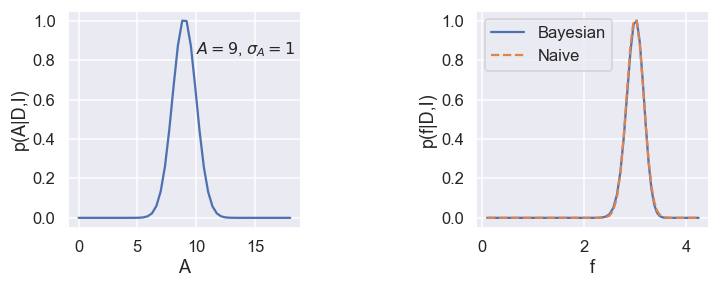
\includegraphics[width=0.7\linewidth]{fig/error_square_root_9_1.png}}
  \caption{
  The left-hand panels show the posterior pdf for the amplitude of a Bragg peak in three different scenarios. The right-hand plots are the corresponding pdfs for the modulus of the structure factor $f=\sqrt{A}$. The solid lines correspond to a full bayesian error propagation, while the dashed lines are obtained with the short-cut error propagation.
  }
\end{figure}
%\clearpage % flush figures 


% !split


\vspace{6mm}

% inline figure
\centerline{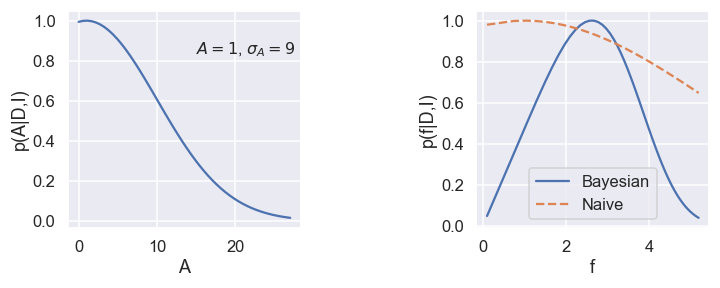
\includegraphics[width=0.7\linewidth]{fig/error_square_root_1_9.png}}

\vspace{6mm}



% !split


\vspace{6mm}

% inline figure
\centerline{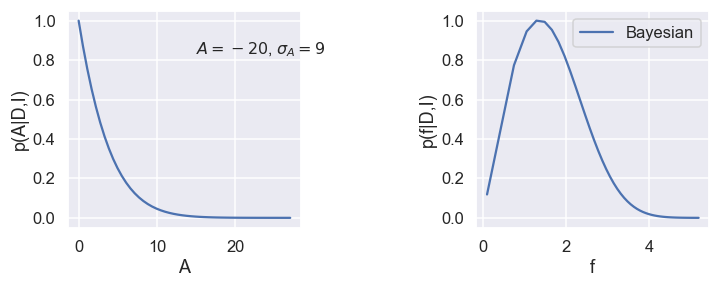
\includegraphics[width=0.7\linewidth]{fig/error_square_root_-20_9.png}}

\vspace{6mm}



% ------------------- end of main content ---------------

% #ifdef PREAMBLE
\end{document}
% #endif

